\documentclass{beamer}

\usepackage{graphicx}
\usepackage{tikz}
\usetikzlibrary{shapes.callouts}
\usepackage{multirow}

%\usetheme{AnnArbor}
%\usetheme{Antibes}
%\usetheme{Bergen}
%\usetheme{Berkeley}
%\usetheme{Berlin}
%\usetheme{Boadilla}
%\usetheme{boxes}
%\usetheme{CambridgeUS}
%\usetheme{Copenhagen}
%\usetheme{Darmstadt}
%\usetheme{default}
%\usetheme{Frankfurt}
%\usetheme{Goettingen}
%\usetheme{Hannover}
%\usetheme{Ilmenau}
%\usetheme{JuanLesPins}
%\usetheme{Luebeck}
%\usetheme{Madrid}
%\usetheme{Malmoe}
%\usetheme{Marburg}
%\usetheme{Montpellier}
%\usetheme{PaloAlto}
%\usetheme{Pittsburgh}
%\usetheme{Rochester}
%\usetheme{Singapore}
%\usetheme{Szeged}
%\usetheme{Warsaw}

\title[EAE105A]{EAE105A \\ Introducci\'on a la Econom\'ia}

\subtitle[Crecimiento Econ\'omico]{Crecimiento Econ\'omico}

\institute[PUC]{Instituto de Econom\'ia\\
Pontificia Universidad Cat\'olica de Chile}

\date[$\:$]

\subject{Mercados y Demanda}

\AtBeginSection[]{
\begin{frame}<beamer>{Contenidos}
\tableofcontents[currentsection, currentsubsection]
\end{frame}}

\begin{document}
\maketitle

\begin{frame}
\frametitle{Introducci\'on}
\begin{itemize}
\setlength\itemsep{1.4em}
\item ?`Por qu\'e nos preocupa el PIB?\\
\begin{itemize}
\item[-] En general, un mayor PIB est\'a vinculado a mejores niveles de vida en un pa\'is.
\end{itemize} 
\item ?`Cambia el PIB? ?`Qu\'e determina el PIB y sus cambios?
\item ?`Qu\'e hace que el PIB entre paises sea distinto?
\item \textbf{Crecimiento econ\'omico}: Se refiere al cambio en el producto de un pa\'is desde un per\'iodo $t$ a $t+1$. 
\end{itemize}
\end{frame}

\begin{frame}
\frametitle{Producto Interno Bruto en el tiempo}
\begin{itemize}
\item Considere las siguientes series del PIB real. 
\end{itemize}
\begin{center}
\begin{figure}
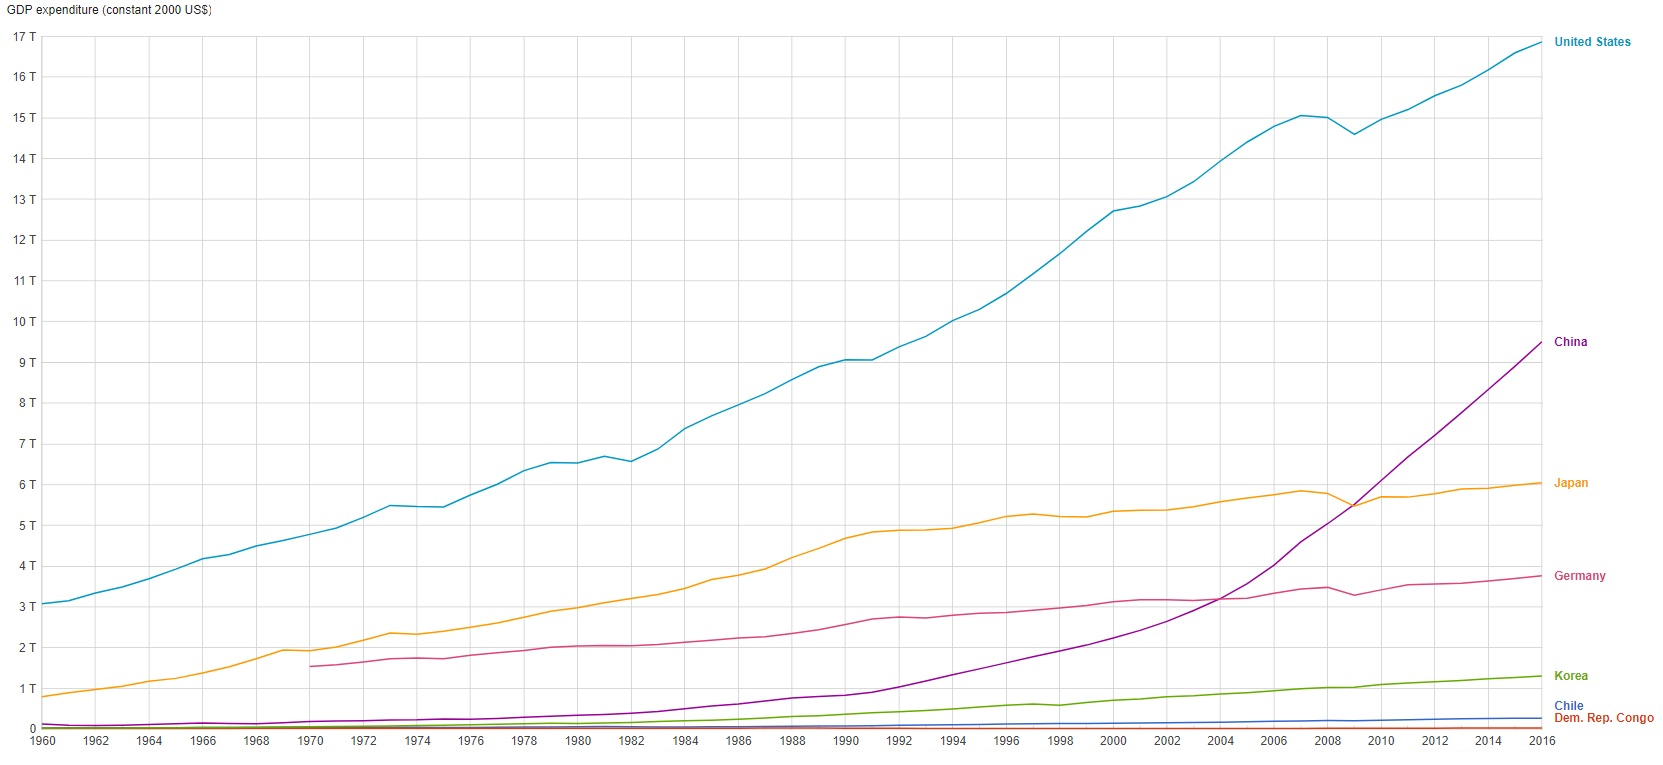
\includegraphics[scale=0.265]{Figuras/PIB}
\end{figure}
\end{center}
\end{frame}

\begin{frame}
\frametitle{Producto Interno Bruto en el tiempo}
\begin{itemize}
\item Considere las siguientes series del PIB real per capita. 
\end{itemize}
\begin{center}
\begin{figure}
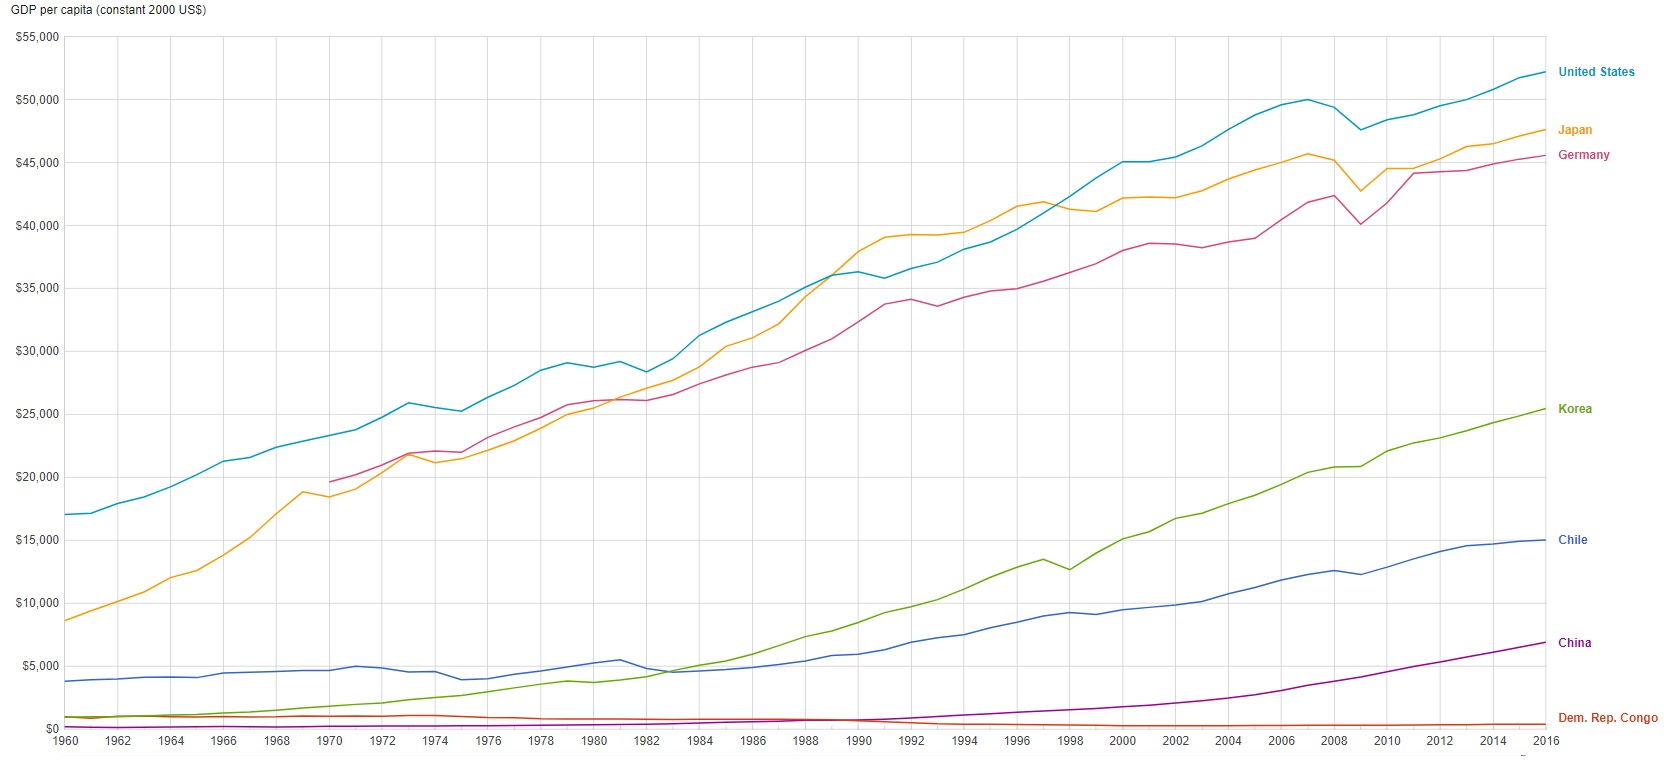
\includegraphics[scale=0.265]{Figuras/PIB2}
\end{figure}
\end{center}
\end{frame}

\begin{frame}
\frametitle{Determinantes del crecimiento - Productividad}
\begin{itemize}
\setlength\itemsep{1.5em}
\item Muchos factores determinan las diferencias de crecimiento econ\'omico entre paises. 
\item La raz\'on fundamental son las diferencias en \textbf{productividad}.
\item \textbf{Productividad}: Cantidad de bienes y servicios producidos por cada unidad de insumo.
\end{itemize}
\end{frame}

\begin{frame}
\frametitle{Determinantes del crecimiento - Productividad}
\begin{itemize}
\setlength\itemsep{1.4em}
\item Recordemos la econom\'ia de Robinson Crusoe.
\item El producto de Robinson depend\'ia de su capacidad de pesca y cosecha de cocos.
\item Si Robinson se hace m\'as productivo (m\'as pescados y cocos por hora de trabajo), su estandar de vida sin duda incrementa.
\item La intuic\'on anterior es an\'aloga para econom\'ias m\'as complejas.
\item ?`Qu\'e cosas est\'an detr\'as de la productividad?
\end{itemize}
\end{frame}

\begin{frame}
\frametitle{Determinantes productividad - Capital f\'isico}
\begin{itemize}
\setlength\itemsep{1.5em}
\item \textbf{Capital F\'isico}: Stock de herramientas y equipos utilizados en la producci\'on de bienes y servicios.
\item Ejemplos: Computadoras, plantas, tractores, camiones, etc...
\item El capital tiene la particularidad de que se puede utilizar para la producci\'on de m\'as unidades de capital.
\end{itemize}
\end{frame}

\begin{frame}
\frametitle{Determinantes productividad - Capital humano}
\begin{itemize}
\setlength\itemsep{1.5em}
\item \textbf{Capital Humano}: Corresponde al conocimiento y las abilidades que los trabajadores emplean a la hora de realizar la producci\'on.
\item El capital humano se adquiere a trav\'es de: Educaci\'on formal, entrenamiento profesional, experiencias previas.
\item Al igual que el capital f\'isico, el capital humano es un insumo de producci\'on producido.
\end{itemize}
\end{frame}

\begin{frame}
\frametitle{Determinantes productividad - Recursos naturales}
\begin{itemize}
\setlength\itemsep{1.0em}
\item \textbf{Recursos naturales}: Insumos de producci\'on provistos por la naturaleza.
\item Ejemplos: R\'ios, dep\'ositos minerales, tierra fertil, viento.
\item En general, los recursos naturales toman dos formas:\\
\begin{itemize}
\setlength\itemsep{0.8em}
\item[-] Renovables: De oferta ilimitada.
\item[-] No renovables: De oferta limitada.
\end{itemize}
\item En ocasiones, diferencias en recursos naturales pueden traducirse en diferencias importantes en productividad.
\end{itemize}
\end{frame}

\begin{frame}
\frametitle{Determinantes productividad - Tecnolog\'ia}
\begin{itemize}
\setlength\itemsep{1.4em}
\item \textbf{Tecnolog\'ia}: Se refiere al conocimiento del uso m\'as eficiente de los insummos disponibles.
\item Algunas formas de conocimiento tecnol\'ogico son de uso p\'ublico. Ej: T\'ecnica de arado.
\item Otras formas son de uso privado. Ej: Patentes, recetas.
\item Es importante reconocer la diferencia entre tecnolog\'ia y capital humano.\\
\begin{itemize}
\setlength\itemsep{0.7em}
\item[-] La primera se refiere al conocimiento disponible.
\item[-] La segunda se refiere al uso de recursos para transmitir dicho conocimiento.
\end{itemize}
\end{itemize}
\end{frame}

\begin{frame}
\frametitle{Pol\'iticas p\'ublicas pro-crecimiento - Ahorro e Inversi\'on}
\begin{itemize}
\setlength\itemsep{1.5em}
\item Los gobiernos pueden aumentar la productividad mediante el \textbf{ahorro y la inversi\'on} en capital.\\
\begin{itemize}
\item[-] Ejemplo: Construcci\'on de carreteras por medio de recursos tributos.
\end{itemize}
\item Lo anterior no est\'a libre de costos: \\
\begin{itemize}
\setlength\itemsep{0.7em}
\item[-] Mayor ahorro e inversi\'on significa menor consumo hoy d\'ia.
\item[-] El capital est\'a sujeto a rendimientos decrecientes.
\end{itemize}
\item El gobierno puede adem\'as indirectamente influenciar las decisiones de ahorro e inversi\'on de los ciudadanos.
\end{itemize}
\end{frame}

\begin{frame}
\frametitle{Pol\'iticas p\'ublicas pro-crecimiento - Inversi\'on Extranjera}
\begin{itemize}
\setlength\itemsep{1.0em}
\item El fomento a la \textbf{inversi\'on exterior} es otra forma en la que los gobiernos pueden fomentar el crecimiento.
\item Dos grandes formas:\\
\begin{itemize}
\setlength\itemsep{0.8em}
\item[-] \textbf{Inversi\'on extranjera directa}: Inversi\'on en territorio dom\'estico de control y recursos externos.
\item[-] \textbf{Inversi\'on portafolio externo}: Inversi\'on operada por recursos externos pero operada a nivel dom\'estico.
\end{itemize}
\item ?`Qu\'e tipo de beneficios provee lo anterior?\\
\begin{itemize}
\setlength\itemsep{0.7em}
\item[-] Construcci\'on de capital f\'isico.
\item[-] Importaci\'on de capital humano y tecnolog\'ia.
\end{itemize}
\end{itemize}
\end{frame}

\begin{frame}
\frametitle{Pol\'iticas p\'ublicas pro-crecimiento - Educaci\'on}
\begin{itemize}
\setlength\itemsep{1.4em}
\item Las \textbf{pol\'iticas pro-educaci\'on} promueven la acumulaci\'on de capital humano y el desarrollo tecnol\'ogico.\\
\begin{itemize}
\item[-] Ejemplo: Ofrecer educaci\'on de calidad y crear conciencia sobre la importancia de educarse.
\end{itemize}
\item Lo anterior no est\'a libre de costos:\\
\begin{itemize}
\setlength\itemsep{0.7em}
\item[-] M\'as individuos estudiando significa menos individuos trabajando.
\item[-] Fuga de cerebros.
\end{itemize}
\end{itemize}
\end{frame}

\begin{frame}
\frametitle{Pol\'iticas p\'ublicas pro-crecimiento - Estabilidad}
\begin{itemize}
\setlength\itemsep{1.4em}
\item Asegurar \textbf{Derechos de propiedad} provee incentivos a invertir.\\
\begin{itemize}
\item[-] Ejemplos: Hacer cumplir contratos, sistema legal s\'olido.
\end{itemize}
\item \textbf{Derechos de propiedad}: Habilidad de un individuo de decidir sobre el uso de los recursos de su propiedad.
\item Una amenaza com\'un a los derechos de propiedad es la inestabilidad pol\'itica.
\end{itemize}
\end{frame}

\begin{frame}
\frametitle{Pol\'iticas p\'ublicas pro-crecimiento - Otros factores}
\begin{itemize}
\item Otros factores importantes:\\
\vspace{2mm}
\begin{itemize}
\setlength\itemsep{1.4em}
\item[-] Instituciones adecuadas.
\item[-] Comercio internacional.
\item[-] Fomento al desarrollo tecnol\'ogico.
\item[-] Crecimiento poblacional.
\end{itemize}
\end{itemize}
\end{frame}




\end{document}
